\subsection{Intermediate Results Compression}\label{sec:match_compress}
The matching results grow exponentially with respect to the size of the graph data.
%TODO:多次提到中间结果指数膨胀,最好在第一次出现的时候说点理由,从别人论文里面摘录出来也行
\textcolor{red}{Consider the matching problem in Figure~\ref{img:running_example},
$S_1$ will generate 28 rows of intermediate results and $S_2$ will generate 8 rows.
And we need $4 \times (28 + 8) = 144$ integers to store them, which is larger than the data graph (10 vertices, 20 edges).
Inspired by the vertex-cover based compression algorithm~\cite{DBLP:journals/pvldb/QiaoZC17},
SeqStar postpones the costly Cartesian product and leveraging equivalence classes among vertices to reduce the size of intermediate results.}
Moreover, we design an on-disk layout that is able to write the compressed data sequentially.

Two techniques are used to compress the intermediate results:
(1) Like VCBC, SeqStar avoids the Cartesian product in the intermediate results.
For each vertex $v$ that will match the root of a star $S$,
SeqStar stores the matched vertices of each neighbor of $v$ in $S$ together as an \emph{image set}.
They are then stored together as a \emph{SuperRow}.
For example, there are two SuperRows in $T_2$ (Figure~\ref{img:running_example}),
each contains a root vertex and two image sets.
(2) SeqStar analyzes the vertices in stars and use equivalence classes to avoid unnecessary storage.
SeqStar first groups the leaf vertices by labels.
It then studies the connections between the leaves and the root.
Vertices have the same edge properties (direction, labels) and filtering function are grouped together as a \emph{neighbor equivalence class},
e.g., $u_2$ and $u_3$ in Figure~\ref{img:running_example}.
The matching results of the vertices are the same, and SeqStar stores their image set only once.
\textcolor{red}{As a result, SeqStar uses only 16 integers to store the compressed intermediate results in Figure~\ref{img:running_example}.}
\begin{figure}[ht]
  \centering
  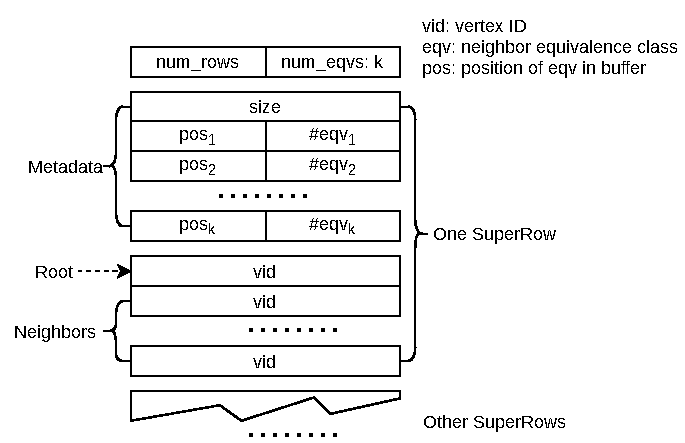
\includegraphics[width=0.45\textwidth]{img/compress.pdf}
  \caption{On-disk layout of the compressed intermediate results.}\label{img:compress}
\end{figure}

Figure~\ref{img:compress} shows the SuperRows' on-disk layout.
In each SuperRow, the matched vertices are stored consecutively.
Metadata $(pos_i, \#eqv_i)$, $ 1 \le i \le k$, are used to store the image sets for each neighbor equivalence class.

\textcolor{red}{In order to reduce the I/O cost for storing SuperRows, matched vertices from the \textsc{NeighborIter} will be appended to the SuperRow file.}

%% VCBC groups the matching results by the vertex-cover and stores the matched vertices in \emph{image sets}.
%% The original data can be restored by doing Cartesian product on the image sets.
%% As a result, only 16 integers are required
%% The compression ratio of the algorithm is as high as $10^{10}$ (\S\ref{sec:experiments_compress}).

% As our experiment shows that a small graph with $10^5$ edges could easily results in $10^{10}$ rows of matching results (Section~\ref{sec:experiments}).
%% Even though we could use stars and auxiliary optimizations to drop out useless matching results as soon as possible, the intermediate results could still be very large.
%% Figure~\ref{img:compress_example} illustrates this phenomenon that a small graph with only 6 vertices could result in 12 rows (48 vertices) of matching results.
%% In the table we could find that $u_1$ and $u_4$ always match the same vertices $v_2$ and $v_1$,
%% whereas the matching results of $u_2$ and $u_3$ are permutations of $v_3, v_4, v_5, v_6$.
%% \emph{The key of the matching result explosion problem is the explosive permutation}.
%% In order to address this problem, we avoid the permutation by postpone the Cartesian production when matching stars, which is similar to VCBC~\cite{DBLP:journals/pvldb/QiaoZC17} but we focus on the compression of property star's matching results for out-of-core systems.

%% Consider Figure~\ref{img:compress_example}, there is a symmetry with $u_2$ and $u_3$.
%% We say that they have the same \textsc{NeighborInfo} or they form a \textsc{NeighborInfo} equivalence class, as they have the same label and same connections to the root $u_4$,
%% and we can be sure that the matching results of $u_2$ and $u_3$ are always same.
%% The \textsc{NeighborInfo} of $u_1$ is different from $u_2$ because $u_1$ has more edges connected to the root.
%% By iterating through the neighbors of $v_1$, we can find the image set for each vertex in the pattern.
%% Instead of permuting the matching vertices, we compress the matching result by just writing down the image sets of each \textsc{NeighborInfo} equivalence class as is shown in the right bottom corner in Figure~\ref{img:compress_example}.
%% And Figure~\ref{img:compress} gives a straightforward disk format to store the compressed star matching results.
%% The final results can be retrieved by doing Cartesian product on the image sets and keeping the unique vertices.
%% We called the compressed data as \emph{SuperRow} since one SuperRow could generate enormous tuples by Cartesian production.
%% \begin{figure}[ht]
%%   \centering
%%   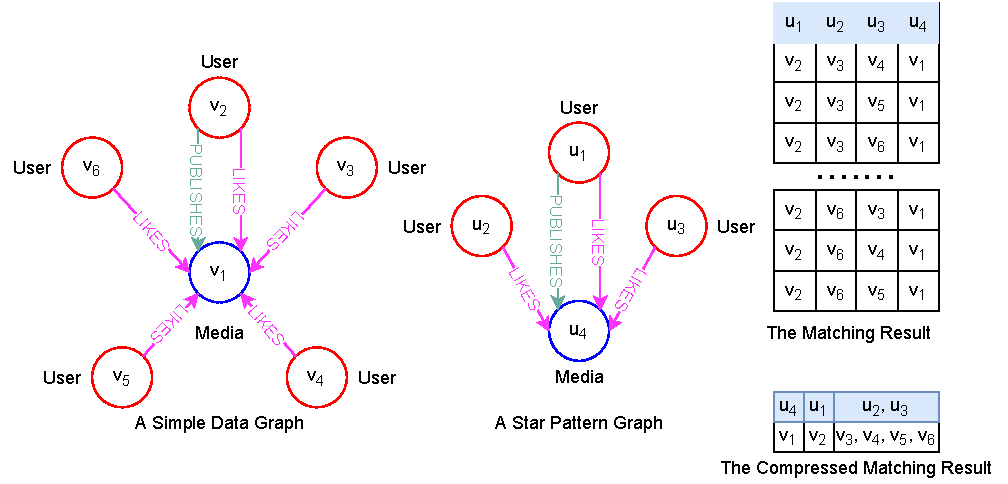
\includegraphics[width=0.53\textwidth]{img/compress_example.pdf}
%%   \caption{A small graph could results in enormous matching results.}\label{img:compress_example}
%% \end{figure}

%% However, there are still two challenges to be faced in practice:
%% 1. In real-world property graphs, as a celebrity vertex could have millions of neighbors, it could become a bottleneck if we have to scan the neighbors multiple times when matching a star;
%% 2. The SuperRows should be written sequentially to reduce the I/O cost.
%% If we want to scan the neighbors only once, we should be able to append the neighbor vertex to the corresponding image set, however, the variable-length image sets make it hard to address these problems.
%% To solve this dilemma, for each SuperRow, we pre-allocate enough space based on the statistical information in the data graph, i.e., the size of neighbors with the \textsc{NeighborInfo}'s label.
%% Thus the vertices could be scanned only once and wrote to the corresponding image set sequentially.
